\chapter{Controlling program flow}
\label{chap:flow}
Non-recursive functions encapsulate code and allow for control of execution flow. That is, if a piece of code needs to be executed many times, then we can encapsulate it in the body of a function, and call the function several times. In this chapter, we will look at more general control of flow via loops and conditional execution. Recursion is another mechanism for controlling flow, but this is deferred to \Cref{sec:recursion}.

\section{While and for loops}
Many programming constructs need to be repeated, and F\# contains many structures for repetition. A \idx[while@\lstinline{while}]{\keyword{while}}-loop has the syntax,
%
\begin{verbatimwrite}{\ebnf/whileLoop.ebnf}
while <*condition*> do <*expr*> [*done*]
\end{verbatimwrite}
\syntax{\ebnf/whileLoop.ebnf}{While loop.}
%
The \idx{condition} \lstinline[language=syntax]{<*condition*>} is an expression that evaluates to true or false. A while-loop repeats the \lstinline[language=syntax]{<*expr*>} expression as long as the condition is true.  Using lightweight syntax the block following the \idx[do@\lstinline{do}]{\keyword{do}} keyword up to and including the \idx[done@\lstinline{done}]{\keyword{done}} keyword may be replaced by a newline and indentation. As an example, the program in \Cref{count} counts from 1 to 10.
%
\fs{countWhile}{Count to 10 with a counter variable.}
%
We will call \lstinline{i} for the counter variable. The counting is done by performing the following computation: In line~\ref{countWhileLoop}, the counter variable is first given an initial value of 1. Then execution enters the while-loop and examines the condition. Since $1 <= 10$ then the condition is true, and execution enters the body of the loop. The body prints the value of the counter to the screen and increases counter by 1. Then execution returns to the top of the while-loop. Now the condition is $2 <= 10$ which is also true, and so execution enters the body and so on until the counter has reach value 11, in which case the condition $11 <= 10$ is false, and execution continues in line~\ref{countWhileContinue}.

In lightweight syntax, this would be as shown in \Cref{countWhileLightweight}.
%
\fs{countWhileLightweight}{Count to 10 with a counter variable using lightweight syntax, see \Cref{countWhile}.}
%
Notice that although the expression following the condition is preceded with a \keyword{do} keyword, and \lstinline[language=syntax]{do <*expr*>} is a do binding, the keyword \keyword{do} is mandatory. 

Counters are so common that a special syntax has been reserved for loops using counters. These are called \idx[for@\lstinline{for}]{\keyword{for}}-loops. For-loops comes in several variants, and here we will focus on the one using an explicit counter. Its syntax is,
%
\begin{verbatimwrite}{\ebnf/forLoop.ebnf}
for <*ident*> = <*firstExpr*> to <*lastExpr*> do <*bodyExpr*> [*done*]
\end{verbatimwrite}
\syntax{\ebnf/forLoop.ebnf}{For loop.}
%
A for-loop initially binds the counter identifier \lstinline[language=syntax]{<*ident*>} to be the value \lstinline[language=syntax]{<*firstExpr*>}. Then execution enters the body and \lstinline[language=syntax]{<*bodyExpr*>} is evaluated. Once done, then the counter is increased and execution evaluates once again \lstinline[language=syntax]{<*bodyExpr*>}. This is repeated until and including the counter has the value \lstinline[language=syntax]{<*lastExpr*>}. As for while-loops, using lightweight syntax the block following the \idx[do@\lstinline{do}]{\keyword{do}} keyword up to and including the \idx[done@\lstinline{done}]{\keyword{done}} keyword may be replaced by a newline and indentation.

The counting example from \Cref{countWhile} using a \keyword{for}-loop is shown in \Cref{count}
%
\fs{count}{Counting from 1 to 10 using a \keyword{for}-loop.}
%
As this interactive script demonstrates, the identifier \lstinline!i! takes all the values between 1 and 10, but in spite of its changing state, it is not mutable. Note also that the return value of the \keyword{for} expression is \lexeme{()} like the \lstinline!printf! functions. The lightweight equivalent is shown in \Cref{countLightweight}.
%
\fs{countLightweight}{Counting from 1 to 10 using a \keyword{for}-loop, see \Cref{count}.}
%

To further compare for- and while-loops, consider the following problem.
\begin{problem}
  Write a program that calculates the $n$'th Fibonacci number.
\end{problem}
The Fibonacci's numbers is a sequence of numbers starting with $1, 1$, and where the next number is calculated as the sum of the previous two. Hence the first ten numbers are: $1, 1, 2, 3, 5, 8, 13, 21, 34, 55$. Fibonacci's numbers are related to Golden spirals shown in \Cref{fig:goldenSpiral}.
\begin{figure}
  \centering
  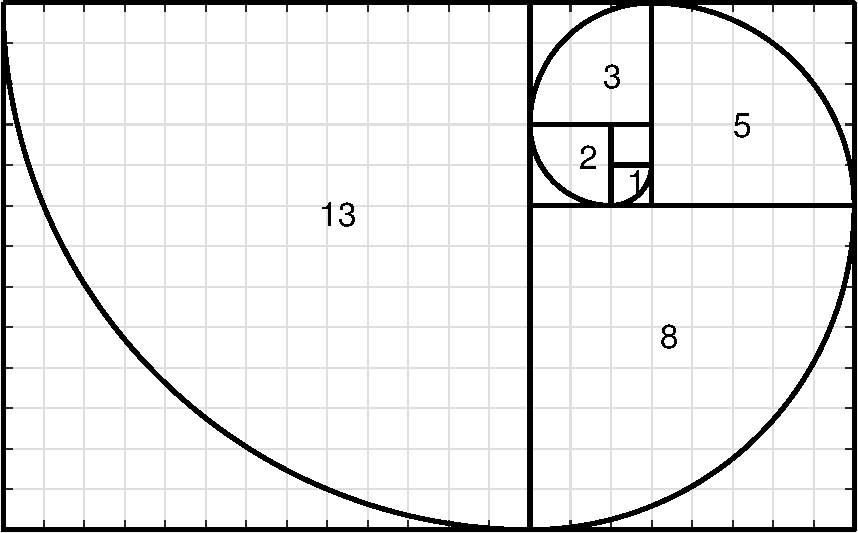
\includegraphics[width=0.45\linewidth]{Fibonacci_spiral}
  \caption{The Fibonacci spiral is an approximation of the golden spiral. Each square has side lengths of successive Fibonacci numbers, and the curve in each square is the circular arc with a radius of the square it is drawn in.}
  \label{fig:goldenSpiral}
\end{figure}
Often the sequence is extended with a preceding number $0$, to be $0, 1, 1, 2, 3, \dots$, which we will do here as well.

We could solve this problem with a \keyword{for}-loop as follows,
%
\fs{fibFor}{The $n$'th Fibonacci number is the sum of the previous 2.}
%
The basic idea of the solution is that if we are given the $(n-1)$'th and $(n-2)$'th numbers, then the $n$'th number is trivial to compute. And assume that $\text{fib}(1)$ and $\text{fib}(2)$ are given, then it is trivial to calculate the $\text{fib}(3)$. For the $\text{fib}(4)$ we only need $\text{fib}(3)$ and $\text{fib}(2)$, hence we may disregard $\text{fib}(1)$. Thus, we realize that we can cyclicly update the previous, current, and next values by shifting values until we have reached the desired $\text{fib}(n)$. This is implement in \Cref{fibFor} as function \lstinline{fib}, which takes an integer \lstinline{n} as argument and returns the $n$'th Fibonacci number. The function does this iteratively using a \keyword{for}-loop, where \lstinline{i} is the counter value, \lstinline{pair} is the pair of the $i-1$'th and $i$'th Fibonacci numbers. In the body of the loop, the $i$'th and $i+1$'th numbers are assigned to \lstinline{pair}. The \keyword{for}-loop automatically updates \lstinline{i} for next iteration. When $n<2$ then the body of the for-loop is not evaluated, and $1$ is returned. This is of course wrong for $n < 1$, but we will ignore this for now.

The same program but using a while-loop is shown in \Cref{fibWhile}.
%
\fs{fibWhile}{Search for the largest Fibonacci number less than a specified number.}
%
As can be seen, the program is almost identical. In this case, the \keyword{for}-loop is to be preferred, since more lines of code typically mean more chances of making a mistake.  However, while-loops are still simpler and possibly easier to argue correctness about. To understand what is being calculated in code such as the while-loop in \Cref{fibWhile}, we can describe the loop in terms of its \idx{loop invariant}. An \idx{invariant} is a statement that is always true at a particular point in a program, and a loop invariant is a statement which is true at the beginning and end of a loop. In line~\ref{fibWhileInvariant} in \Cref{fibWhile}, we may state the invariant: The variable \lstinline{pair} is the pair of the $i-1$'th and $i$'th Fibonacci numbers. This is provable by induction:
\begin{description}
\item[Base case:]  Before entering the while loop, \lstinline{i} is 1, \lstinline{pair} is (0, 1). Thus, the invariant is true.
\item[Induction step:] Assuming that \lstinline{pair} is the $i-1$'th and $i$'th Fibonacci numbers, then the body first assigns a new value to \lstinline{pair} as the $i$'th and $i+1$'th Fibonacci numbers, then increases $i$ with one such that at the end of the loop the \lstinline{pair} again contains the the $i-1$'th and $i$'th Fibonacci numbers. Thus, the invariant is true.
\end{description}
Thus when know that the second value in \lstinline{pair} holds the value of the $i$'th Fibonacci number, and since we further may prove that when line~\ref{fibWhileInvariantContinue} is only reached, then $i = n$, and thus that \lstinline{fib} returns the $n$'th Fibonacci number. 

While-loops also allows for other logical structures than for-loops, such as the case when the number of iteration cannot easily be decided when entering the loop. As an example, consider a slight variation of the above problem, where we wish to find the largest Fibonacci number less than some number. A solution to this problem is shown in \Cref{fibWhileLargest}.
%
\fs{fibWhileLargest}{Search for the largest Fibonacci number less than a specified number.}
%
The strategy here is to iteratively calculate numbers in Fibonacci's sequence until we've found one larger than the argument \lstinline{n}, and then return the previous. This could not be calculated with a for-loop.

\section{Conditional expressions}
Programs often contains code, which only should be executed under certain conditions. This can be expressed as \keyword{if}-expressions, whos syntax is as follows.\idxs{if@\lstinline{if}}\idxs{then@\lstinline{then}}\idxs{elif@\lstinline{elif}}\idxs{else@\lstinline{else}}
%
\begin{verbatimwrite}{\ebnf/conditional.ebnf}
if <*cond*> then <*expr*> {*elif <*cond*> then <*expr*>*} [*else <*expr*>*]
\end{verbatimwrite}
\syntax{\ebnf/conditional.ebnf}{Conditional expressions.}
%
The condition \lstinline[language=syntax]{<*con*>} is an expression resulting in a Boolean value, and there can be zero or more \keyword{elif} conditions as indicated by \lstinline[language=syntax]{{**}}. Each expression \lstinline[language=syntax]{<*expr*>}  is called a \idx{branch}, and all branches must have the identical type, such that regardless which branch is chosen, then the type of the result of the conditional expression is the same. The result of the conditional expression is the first branch, for which its condition was true and if all conditions are false then the \keyword{else}-branch is evaluated. If no \keyword{else} expression is present, then \lexeme{()} will be returned. See \Cref{condition} for a simple example.
%
\fs{condition}{Conditions evaluates their branches depending on the value of the condition.}
%
The lightweight syntax allows for newlines entered everywhere, but indentation must be used to express scope. 

To demonstrate conditional expressions, let us write a program, which writes the sentence, ``I have n apple(s)'', where the plural 's' is added appropriately for various $n$s. This is done in \Cref{conditionalLightweight} using the lightweight syntax.
%
\fs{conditionalLightweight}{Using conditional expression to generate different strings.}
%
The sentence structure and its variants give rise to a more compact solution since the language to be returned to the user is a variant of "I have/or no/number apple(s)", i.e., under certain conditions should the sentence use ``have'' and ``owe'' etc. So, we could instead make decisions on each of these sentence parts and then built the final sentence from its parts. This is accomplished in the following example:
%
\fs{conditionalLightweightAlt}{Using sentence parts to construct the final sentence.}
%
While arguably shorter, this solution is also denser, and for a small problem like this, it is most likely more difficult to debug and maintain.

Note that both \keyword{elif} and \keyword{else} branches are optional, which may cause problems. For example, both \mbox{\lstinline!let a = if true then 3!} and \mbox{\lstinline!let a = if true then 3 elif false then 4!}  will be invalid, since F\# is not smart enough to realize that the type of the expression is uniquely determined. Instead, F\# looks for the \keyword{else} to ensure all cases have been covered, and that \lstinline!a! always will be given a unique value of the same type regardless of the branch taken in the conditional statement, hence, \mbox{\lstinline!let a = if true then 3 else 4!}  is the only valid expression of the 3. In practice, F\# assumes that the omitted branch returns \lexeme{()}, and thus it is fine to say \mbox{\lstinline!let a = if true then ()!} and \mbox{\lstinline!if true then printfn "hej"!}. Nevertheless, it is good practice in F\# always to include an \keyword{else} branch.

\section{Programming intermezzo: Automatic conversion of decimal to binary numbers}
Using loops and conditional expressions, we are now able to solve the following problem:
\begin{problem}
  Given an integer on decimal form, write its equivalent value on the binary form.
\end{problem}
To solve this problem, consider odd numbers: They all have the property, that the least significant bit is 1, e.g., $1_2 = 1, 101_2 = 5$ in contrast to even numbers such as $110_2 = 6$. Division by 2 is equal to right-shifting by 1, e.g., $1_2/2 = 0.1_2 = 0.5, 101_2/2 = 10.1_2 = 2.5, 110_2/2 = 11_2 = 3$. Thus, by integer division by 2 and checking the remainder, we may sequentially read off the least significant bit. This leads to the algorithm shown in \Cref{dec2bin}.
%
\fs{dec2bin}{Using integer division and remainder to write any positive integer on binary form.}
%
In the code, the states \lstinline!v! and \lstinline!str! are iteratively updated until \lstinline!str! finally contains the desired solution.

To prove that \Cref{dec2bin} calculates the correct sequence we use induction. First we realize, that for $v < 1$ then the \keyword{while} loop is skipped, and the result is trivially true. We will concentrate on line~\ref{dec2binWhile} in \Cref{dec2bin}, and we will prove the following loop invariant: The string \lstinline{str} contains all the bits of \lstinline{n} to the right of the bit pattern remaining in variable \lstinline{v}.
\begin{description}
\item[Base case $n=000\ldots000x$:] If $n$ only uses the lowest bit then $n=0$ or $n=1$. If $n=0$ then it is trivially correct. Considering the case $n=1$: Before entering into the loop, \lstinline{v} is 1, \lstinline{str} is the empty string, so the invariant is true. The condition of the while-loop is $1>0$ so execution enters the loop. Since integer division of 1 by 2 gives 0 with remainder 1, then \lstinline{str} is set to \lstinline{"1"} and \lstinline{v} to 0. Now we reexamine the while-loop's condition, $0>0$, which is false, so we exit the loop. At this point, \lstinline{v} is 0 and \lstinline{str} is \lstinline{"1"}, so all bits have been shifted from \lstinline{n} to \lstinline{str} and none are left in \lstinline{v}. Thus the invariant is true. Finally, the program returns \lstinline{"0b1"}.
\item[Induction step:] Consider the case of $n>1$, and assume that the invariant is true when entering the loop, i.e., that $m$ bits already have been shifted to \lstinline{str} and that $n>2^m$. In this case \lstinline{v} contains the remaining bits of \lstinline{n}, which is the integer division \lstinline{v = n / 2**m}. Since $n>2^m$ then \lstinline{v} is non-zero and the loop conditions is true, so we enter the loop body. In the loop body we concatenate the rightmost bit of \lstinline{v} to the left of \lstinline{str} using \lstinline{v % 2}, %
and right-shift \lstinline{v} one bit to the right with \lstinline{v <- v / 2}. Thus, when returning to the condition, the invariant is true, since the right-most bit in \lstinline{v} has been shifted to \lstinline{str}. This continues until all bits have been shifted to \lstinline{str} and \lstinline{v = 0}, in which case the loop terminates, and \lstinline{"0b"+str} is returned.
\end{description}
Thus we have proven, that \lstinline{dec2bin} correctly converts integers to strings representing binary numbers.

%%% Local Variables:
%%% TeX-master: "fsharpNotes"
%%% End:

